\documentclass{fancyslides} 
\usepackage[utf8]{inputenc}
\usepackage{times}


\graphicspath{{img/}}

%%% Beamer settings (do not change)
\usetheme{default} 
\setbeamertemplate{navigation symbols}{} %no navigation symbols
\setbeamercolor{structure}{fg=\yourowntexcol} 
\setbeamercolor{normal text}{fg=\yourowntexcol} 



%%%%%%%%%%%%%%%%%%%%%%%%%
%%% CUSTOMISATIONS %%%%%%
%%%%%%%%%%%%%%%%%%%%%%%%%


%%%% SLIDE ELEMENTS
\newcommand{\structureopacity}{0.75} %opacity for the structure elements (boxes and dots)
\newcommand{\strcolor}{black} %elements colour (predefined blue; orange; green)

%%%% TEXT COLOUR
\newcommand{\yourowntexcol}{white}


%%%%%%%%%%%%%%%%%%%%%%%%%
%%% TITLE SLIDE DATA %%%%
%%%%%%%%%%%%%%%%%%%%%%%%%
\fbckg{abstract-data}
\newcommand{\titlephrase}{On-Line Analytical Processing}
\newcommand{\name}{Javier Bonet \\ Joel Catacora \\}
\newcommand{\affil}{Base de datos avanzada}
\newcommand{\email}{22 de abril del 2015}


\begin{document}


\startingslide %this generates titlepage from the data above

\fbckg{white}
\begin{frame}
\pointedsl{{\LARGE ¿Qué es OLAP?}}
\end{frame}


\fbckg{white}
\begin{frame}
\misc
{
El \textbf{procesamiento analítico en línea} (OLAP) es una solución utilizada en el campo de la inteligencia de negocios, cuyo objetivo es permitir la consulta de grandes cantidades de datos de forma eficiente y sencilla.
}
\end{frame}

\fbckg{white}
\begin{frame}
\misc
{
El concepto OLAP puede ser definido con solo 5 palabras: Análisis Rápido de Información Compartida Multidimensional, (Fast Analysis of Shared Multidimensional Information, o FASMI).
}
\end{frame}

\fbckg{white}
\begin{frame}
\misc
{
\begin{itemize}
  \item \textbf{Rápida}: el sistema está dirigido a proporcionar la mayoría de las respuestas a los usuarios en pocos segundos.
  \item \textbf{Análisis}: el sistema puede hacer frente a cualquier lógica de negocio y análisis estadístico que sea relevante para el usuario, en forma relativamente sencilla.
  \item \textbf{Compartida}: significa que el sistema implementa todos los requisitos de seguridad de la confidencialidad.
  \item \textbf{Multidimensionalidad}: el sistema debe proveer una vista conceptual multidimensional de los datos.
  \item \textbf{Información}: se refiere a todos los datos y la información derivada, que sea relevante para la aplicación.
\end{itemize}
}
\end{frame}



\fbckg{white}
\begin{frame}
\pointedsl{{\LARGE Características}}
\end{frame}


\fbckg{white}
\begin{frame}
\itemized{
\item \textbf{Visión multidimensional de los datos}
}
\end{frame}

\fbckg{white}
\begin{frame}
\itemized{
\item \textbf{Visión multidimensional de los datos}
\item \textbf{Soporta cálculos complejos}
}
\end{frame}

\fbckg{white}
\begin{frame}
\itemized{
\item \textbf{Visión multidimensional de los datos}
\item \textbf{Soporta cálculos complejos}
\item \textbf{Inteligencia respecto del tiempo}
}
\end{frame}


\fbckg{white}
\begin{frame}
\pointedsl{{\LARGE Reglas de Codd}}
\end{frame}

\fbckg{white}
\begin{frame}
\itemized{
\item \textbf{Visión multidimensional}
}
\end{frame}

\fbckg{white}
\begin{frame}
\itemized{
\item \textbf{Visión multidimensional}
\item \textbf{Manipulación intuitiva de los datos}
}
\end{frame}

\fbckg{white}
\begin{frame}
\itemized{
\item \textbf{Visión multidimensional}
\item \textbf{Manipulación intuitiva de los datos}
\item \textbf{Accesibilidad}
}
\end{frame}

\fbckg{white}
\begin{frame}
\itemized{
\item \textbf{Visión multidimensional}
\item \textbf{Manipulación intuitiva de los datos}
\item \textbf{Accesibilidad}
\item \textbf{Soporte multi-usuario}
}
\end{frame}

\fbckg{white}
\begin{frame}
\itemized{
\item \textbf{Visión multidimensional}
\item \textbf{Manipulación intuitiva de los datos}
\item \textbf{Accesibilidad}
\item \textbf{Soporte multi-usuario}
\item \textbf{Mantener la información separada del origen de datos}
}
\end{frame}

\fbckg{white}
\begin{frame}
\itemized{
\item \textbf{Visión multidimensional}
\item \textbf{Manipulación intuitiva de los datos}
\item \textbf{Accesibilidad}
\item \textbf{Soporte multi-usuario}
\item \textbf{Mantener la información separada del origen de datos}
\item \textbf{Rendimiento uniforme}
}
\end{frame}

\fbckg{white}
\begin{frame}
\itemized{
\item \textbf{Visión multidimensional}
\item \textbf{Manipulación intuitiva de los datos}
\item \textbf{Accesibilidad}
\item \textbf{Soporte multi-usuario}
\item \textbf{Mantener la información separada del origen de datos}
\item \textbf{Rendimiento uniforme}
\item \textbf{Dimensiones y niveles de agregación ilimitados}
}
\end{frame}


\fbckg{white}
\begin{frame}
\pointedsl{\LARGE{Agregaciones}}
\end{frame}

\fbckg{white}
\begin{frame}
\misc
{
Los \textbf{agregados} se utilizan en los modelos dimensionales del Data Warehouse para producir efectos positivos sobre el tiempo que toma una consulta sobre grandes conjuntos de datos. El uso más común de los agregados es tomar una dimensión y cambiar su granularidad.
Al cambiar la granularidad de la dimensión, la tabla de hechos tiene que ser parcialmente resumida para adaptarse a la nueva dimensión, creando así nuevas tablas de dimendiones y de hecho, que encajan en este nuevo nivel de granularidad. 
}
\end{frame}

\fbckg{white}
\begin{frame}
\misc
{
\textbf{Ejemplo}

Este esquema copo de nieve, tiene una sola tabla de echos \textit{Sales}, dos métricas (\textit{units and dollars}) y cuatro tablas de dimensiones (\textit{Product, Mfr, Customer, Time, y Customer}).

\begin{center}
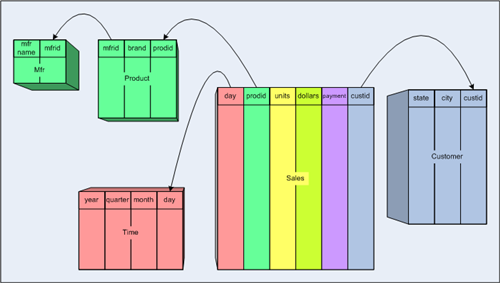
\includegraphics[scale=0.5]{aggregate_tables_1}
\end{center}
}
\end{frame}

\fbckg{white}
\begin{frame}
\misc
{
\textbf{Ejemplo}

Creamos una tabla agregada, Agg\_1:
 
\begin{center}
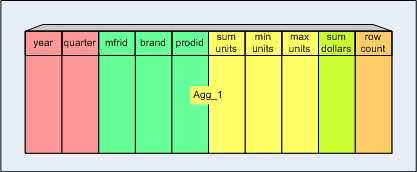
\includegraphics[scale=0.5]{aggregate_tables_2}
\end{center}
}
\end{frame}

\fbckg{white}
\begin{frame}
\misc
{Veamos como las columnas del esquema original se han combinado en la tabla Agg\_1:

\begin{itemize}
  \item La dimensión \textit{Time} se "colapsó" en la tabla de agregación, omitiendo las columnas \textit{month} y \textit{day}.
  \item Las dos tablas de la dimensión \textit{Product} se "colapsaron" en la tabla de agregación.
  \item La dimensión \textit{Customer} se "perdió".
  \item Para cada métrica en la tabla de hechos (\textit{units, dollars}), hay uno o más métricas en la tabla de agregación (\textit{sum units, min units, max units, sum dollars}).
  \item También hay una nueva métrica, \textit{row count}, que representa la métrica "conteo".
\end{itemize}
}
\end{frame}


\fbckg{white}
\begin{frame}
\misc
{
\textbf{Ejemplo}

Otra tabla agregada, Agg\_2:

\begin{center}
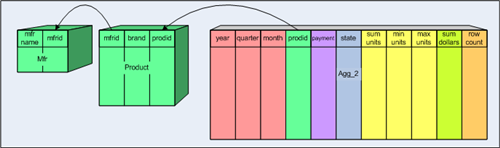
\includegraphics[scale=0.6]{aggregate_tables_3}
\end{center}

Varias dimensiones colapsaron: \textit{Time} en el nivel \textit{Quarter}; \textit{Customer} en el nivel \textit{State};
y \textit{Payment Method} a nivel \textit{Payment Method}. Pero la dimensión \textit{Product} se conservó.}
\end{frame}


\fbckg{white}
\begin{frame}
\pointedsl{\LARGE{Hipercubo de datos}}
\end{frame}

\fbckg{white}
\begin{frame}
\misc
{
El cubo OLAP puede ser pensado como una extensión de la matriz multidimensional de una hoja de cálculo, de ahí el nombre del hipercubo. Técnicamente, el cubo de datos es una representación multidimensional de datos, junto con todos los agregados posible, es decir, los agregados que resultan mediante la selección de un subconjunto propio de las dimensiones y sumando sobre todas las dimensiones restantes.
}
\end{frame}

\fbckg{white}
\begin{frame}
\misc
{
Un cubo OLAP es una representación abstracta de la proyección de una relación de un RDBMS (Sistema administrador de bases de datos relacionales).
Dada una relación de orden N, tenemos una proyección que dispone de los campos X, Y, Z como clave de la relación y de W como atributo residual.
Categorizando esto como una función se tiene que:
$f : (X,Y,Z) \rightarrow  W$

Los atributos X, Y, Z se corresponden con los ejes del cubo, mientras que el valor de W devuelto por cada tripleta (X, Y, Z) se corresponde con el dato o elemento que se rellena en cada celda del cubo.

}
\end{frame}

\end{document}
